\documentclass[t,13pt,graphics=pdflatex,xcolor=table,aspectratio=43]{beamer}

%% Misc packaging
\usepackage[utf8]{inputenc}
\usepackage[T2A]{fontenc}
\usepackage[english,main=russian]{babel}
\usepackage{amssymb,amsmath}
\usepackage{graphicx}
\usepackage{multirow}

%% Добавляйте новые пути с картинками в эту команду.
%% Будет примерно так:
%% \graphicspath{{itmo-logo/}{pic/}}
\graphicspath{{itmo-logo/}}

%% ИТМОшные цвета
\definecolor{itmoblue}{RGB}{25,70,186}
\definecolor{itmored}{RGB}{236,11,67}

%% Установка основных цветов в тексте
\setbeamercolor{normal text}{fg=itmoblue}
\setbeamercolor{alerted text}{fg=itmored}
\setbeamercolor{frametitle}{fg=white}
\setbeamercolor{palette quaternary}{fg=white,bg=itmoblue}
\setbeamercolor{frametitle}{bg=itmoblue}

%% Дизайн заголовка обычного слайда
\setbeamertemplate{frametitle}{
\begin{beamercolorbox}[ht=0.15\textheight,wd=\paperwidth]{frametitle}
    \begin{minipage}[b][0.15\textheight][t]{0.35\paperwidth}
    
\includegraphics[width=\textwidth]{itmo_horiz_blue_rus.png}
    \end{minipage}~\begin{minipage}[b][0.15\textheight][c]{0.6\paperwidth}
    \begin{flushright}\normalsize\insertframetitle\end{flushright}
    \end{minipage}
\end{beamercolorbox}
}
\beamertemplatenavigationsymbolsempty


%% Хрень всякая
\newcommand{\alertAt}[2]{\alt<#1>{\alert{#2}}{#2}}

\begin{document}

%% Идиотский способ сделать титульную страницу
\begingroup
\setbeamercolor{background canvas}{bg=itmoblue}
\setbeamercolor{normal text}{fg=white}
\begin{frame}[plain]
\color{white}
\centering\bfseries

\includegraphics[width=0.35\textwidth]{itmo_small_blue_rus.png}

{\Large {<<}Анализ и разработка алгоритмов \par
            сжатия коротких текстов{>>} \par}

\vspace{0pt plus 0.3filll}

{\large Минаев Борис Юрьевич}

\vspace{0pt plus 0.3filll}

{\small Научный руководитель:\par
 канд. техн. наук, доцент Буздалов Максим Викторович}

\vspace{0pt plus 0.3filll}

{\small Кафедра КТ\par 2017} 

\vspace{0pt plus 1filll}
\end{frame}
\endgroup



\addtobeamertemplate{navigation symbols}{}{%
    \usebeamerfont{footline}%
    \usebeamercolor[fg]{footline}%
    \hspace{1em}%
    \insertframenumber/\inserttotalframenumber
}

\begin{frame}{Постановка задачи}
\begin{itemize}
    \item Реализовать алгоритм сжатия сообщений
    \item Каждое сообщение длиной в среднем 30 символов
    \item Необходимо уметь разжимать отдельные сообщения
    \item Можно заранее предподсчитать общую дополнительную информацию
\end{itemize}
\end{frame}

\begin{frame}{Актуальность задачи}
\begin{itemize}
    \item Алгоритм разрабатывался для хранения сообщений в социальной сети ВКонтакте
    \item 5 миллиардов сообщений в сутки
    \item 4 триллиона сообщений всего
    \item 400 терабайт данных
    \item Хотим использовать как можно меньше серверов, но при этом хранить как можно больше сообщений в оперативной памяти
\end{itemize}
\end{frame}

\begin{frame}{Распределение сообщений по длинам}
\begin{center}
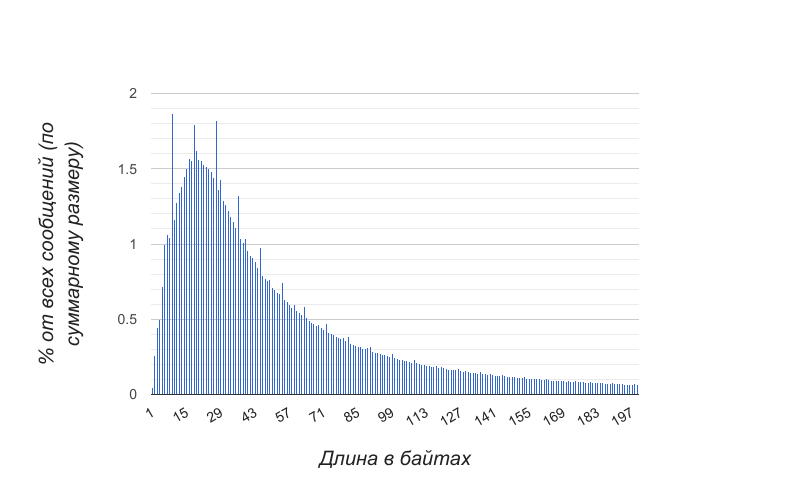
\includegraphics[width=4.4in]{pics/msgs-len.png}
\end{center}
\end{frame}


\begin{frame}{Существующие решения}
\begin{itemize}
    \item Большинство алгоритмов сжатия работают хорошо только на длинных текстах
    \item На коротких сообщениях они не успевают обучиться
    \item Вывод: нужно использовать алгоритм, который можно <<обучить>> на старых сообщениях
\end{itemize}
\end{frame}


\begin{frame}{Оценка качества алгоритма}
\begin{center}
$ \text{compression ratio} = \frac{\text{messages size}}{\text{compressed messages size} + \text{additional info}} $
\end{center}
\begin{itemize}
    \item messages size~--- суммарный размер сообщений, которые помещаются в оперативную память
    \item compressed messages size~--- суммарный размер сообщений в сжатом виде
    \item additional info~--- размер дополнительной информации, которую надо хранить, чтобы уметь разжимать сообщения
\end{itemize}
\end{frame}

\begin{frame}{Набор данных для тестирования}    
\begin{itemize}
    \item Случайные русскоязычные твиты
    \item получены с помощью twitter streaming API
    \item 250 мегабайт
    \item 2 миллиона сообщений
\end{itemize}
\end{frame}


\begin{frame}{LZW}    
\begin{itemize}
    \item Храним набор подстрок
    \item Находим самую длинную подстроку $W$, которую уже видели
    \item Добавляем в словарь подстроку $W + \text{последний символ}$
    \item Словарь фиксированного размера (использовался $2^{20}$)
    \item При переполнении удаляем подстроки по LRU
    \item Коэффициент сжатия = 2.14
\end{itemize}
\end{frame}

\begin{frame}{Однобуквенный Хаффман}    
\begin{itemize}
    \item Считаем вероятность каждого символа
    \item Строим дерево Хаффмана с 256 листьями
    \item Коэффициент сжатия = 1.37
\end{itemize}
\end{frame}

\begin{frame}{Хаффман по словам}    
\begin{itemize}
    \item Разбиваем все символы на буквы и все остальные знаки
    \item Каждое сообщение разбивается на слова и разделители
    \item Отдельно строим словарь <<слов>> и словарь <<разделителей>>
    \item Для каждого словаря строим дерево Хаффмана
    \item Чтобы деревья не были слишком большими, удаляем слова, которые встречаются мало раз и добавляем слово-исключение
    \item Чтобы закодировать слово, которого нет в словаре, записываем слово-исключение, а потом побайтово нужное слово
    \item Коэффициент сжатия = 2.57
    \item \alertAt{2}{Проблема: 3\% слов, которые не попали в словарь, генерируют 13\% сжатых данных!}
\end{itemize}
\end{frame}

\begin{frame}{Хаффман по словам + Однобуквенный Хаффман}    
\begin{itemize}
    \item Делаем Хаффман по словам
    \item Чтобы закодировать слово, которого нет в словаре, записываем слово-исключение, а потом однобуквенным Хаффманом кодируем слово (предварительно посчитав вероятности букв)
    \item Коэффициент сжатия = 2.72
\end{itemize}
\end{frame}

\begin{frame}{Хаффман по словам + Однобуквенный Хаффман зависящий от предыдущей буквы}    
\begin{itemize}
    \item Делаем Хаффман по словам
    \item Чтобы закодировать слово, которого нет в словаре, записываем слово-исключение, а потом кодируем следующим образом:
    \item Посчитаем для каждого символа вероятность встретить каждый другой символ после него. Построим на этих вероятностях 256 различных деревьев Хаффмана. Будем использовать их для кодирования.
    \item Коэффициент сжатия = 2.82
    \item 6\% слов, которые не попали в словарь, генерируют 12\% сжатых данных
\end{itemize}
\end{frame}

\begin{frame}{Сравнение}
\begin{center}
\begin{tabular}{| p{5cm} | l |}
    \hline 
    Алгоритм & Коэффициент сжатия \\
    \hline 
    LZW & 2.14 \\
    \hline 
    Однобуквенный Хаффман & 1.37 \\
    \hline 
    Хаффман по словам & 2.57 \\
    \hline 
    Хаффман по словам + Однобуквенный Хаффман & 2.72 \\
    \hline 
    Хаффман по словам + Однобуквенный Хаффман зависящий от предыдущей буквы & 2.82 \\
    \hline 
    gzip всех сообщений целиком (не применим) & 2.95 \\
    \hline
\end{tabular}
\end{center}
\end{frame}

\begin{frame}{Сравнение на реальных данных. LZW}
\begin{center}
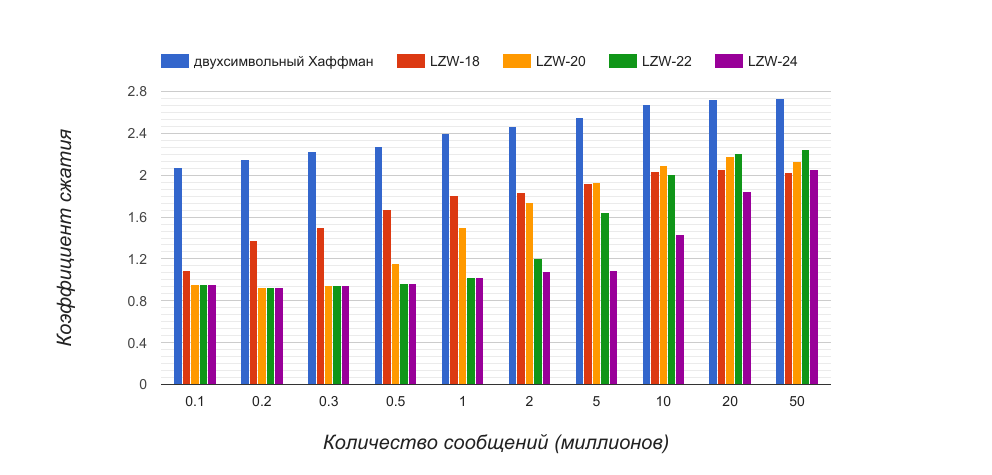
\includegraphics[height=2.2in]{pics/lzw.png}
\end{center}
\end{frame}


\begin{frame}{Сравнение на реальных данных. Хаффман}
\begin{center}
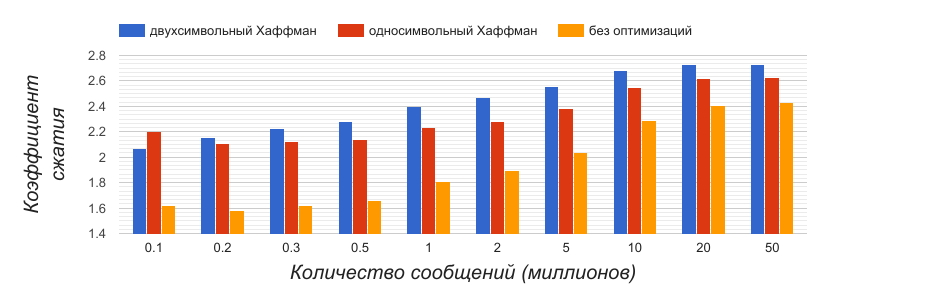
\includegraphics[width=5in]{pics/compare.png}
\end{center}
\end{frame}



\begin{frame}{Выводы}    
\begin{itemize}
    \item Разработан алгоритм сжатия коротких текстов на основе уже существующих алгоритмов сжатия
    \item Основное отличие алгоритма~--- возможность быстро разжимать отдельные сообщения
    \item По эффективности алгоритм не сильно проигрывает архиваторам, которые сжимают текст целиком
    \item Алгоритм уже применяется для сжатия сообщений в социальной сети ВКонтакте, что позволило сэкономить несколько терабайт оперативной памяти
\end{itemize}
\end{frame}

\begin{frame}[plain, c]{Вопросы}    
\begin{center}
\Huge Вопросы?
\end{center}
\end{frame}



\end{document}
